\documentclass[conference]{IEEEtran}
\IEEEoverridecommandlockouts
% The preceding line is only needed to identify funding in the first footnote. If that is unneeded, please comment it out.
\usepackage{cite}
\usepackage[utf8]{inputenc}
\usepackage{amsmath,amssymb,amsfonts}
\usepackage{algorithmic}
\usepackage{graphicx}
\usepackage{textcomp}
\usepackage{xcolor}
\def\BibTeX{{\rm B\kern-.05em{\sc i\kern-.025em b}\kern-.08em
    T\kern-.1667em\lower.7ex\hbox{E}\kern-.125emX}}
\begin{document}

\title{Lightweight solution to background noise in crowd counting\\
% {\footnotesize \textsuperscript{*}Note: Sub-titles are not captured in Xplore and
% should not be used}
% \thanks{Identify applicable funding agency here. If none, delete this.}
}

\author{\IEEEauthorblockN{Thien Thai}
\IEEEauthorblockA{\textit{Faculty of Information Technology} \\
\textit{VNUHCM-University of Science}\\
Ho Chi Minh City, Vietnam \\
tthien@apcs.vn}
\and
\IEEEauthorblockN{Ngoc Quoc Ly}
\IEEEauthorblockA{\textit{Faculty of Information Technology} \\
\textit{VNUHCM-University of Science}\\
Ho Chi Minh City, Vietnam \\
lqngoc@fit.hcmus.edu.vn}
% \and
% \IEEEauthorblockN{3\textsuperscript{rd} Given Name Surname}
% \IEEEauthorblockA{\textit{dept. name of organization (of Aff.)} \\
% \textit{name of organization (of Aff.)}\\
% City, Country \\
% email address or ORCID}
% \and
% \IEEEauthorblockN{4\textsuperscript{th} Given Name Surname}
% \IEEEauthorblockA{\textit{dept. name of organization (of Aff.)} \\
% \textit{name of organization (of Aff.)}\\
% City, Country \\
% email address or ORCID}
% \and
% \IEEEauthorblockN{5\textsuperscript{th} Given Name Surname}
% \IEEEauthorblockA{\textit{dept. name of organization (of Aff.)} \\
% \textit{name of organization (of Aff.)}\\
% City, Country \\
% email address or ORCID}
% \and
% \IEEEauthorblockN{6\textsuperscript{th} Given Name Surname}
% \IEEEauthorblockA{\textit{dept. name of organization (of Aff.)} \\
% \textit{name of organization (of Aff.)}\\
% City, Country \\
% email address or ORCID}
}

\maketitle

% \begin{abstract}
% In this paper, we have proposed an enhancement of lightweight C-CNN, called DCCNN, to compensate for its lack of mechanisms to alleviate background noise using dilated convolution and average pooling. DCCNN performance improves significantly on medium and spared crowd scenes in ShanghaiTech part B dataset, achieves an 18\% lower MAE comparing to C-CNN while keeps no significant impact on computation cost. We conduct a series of benchmarks on both models to compare their performance and efficiency. 
% \end{abstract}

\begin{abstract}
This paper proposed Dilated Compact Convolutional Neural Network (DCCNN) for single-image crowd density estimation from the original lightweight C-CNN.  DCCNN is an enhancement of lightweight C-CNN compensated for lack of mechanisms to alleviate background noise using dilated convolution and average pooling. The performance of our proposed model improves significantly on medium and spared crowd scenes in ShanghaiTech part B dataset, achieving 18\% lower MAE compared to C-CNN while requiring virtually no additional computational costs.
\end{abstract}

\begin{IEEEkeywords}
crowd counting, crowd density estimation, dilated
convolution, deep learning
\end{IEEEkeywords}

% \section{Introduction}
\section{Introduction}

With the development of urbanization and mass surveillance, automated crowd scene understanding, with crowd counting as a sub-problem, become in-demand. Single-image crowd counting in computer vision is the process to automatically count the number of people in an image using a computer.  The topic of single-image crowd counting remain challenging.

Recent works on crowd counting focus on tackle two main challenges: Scale variation caused by perspective distortion and background noise. Despite state-of-the-art works robust to both the above challenges, their models are too complex and resource hungry \cite{liu2019context, jiang2019crowd, liu2019adcrowdnet, amirgholipour2020pdanet}. C-CNN \cite{9053780} was proposed as a lightweight approach. However, C-CNN does not cover all problems of crowd counting.

In this paper, we show that C-CNN performance can be improve significant without increase on model complexity. 






 

% related work
\section{Related work}
\subsection{Traditional method}
Originally, total people in the crowd were count by detection. The method in this group mostly using a sliding window with a classifier trained on low-level hand-craft features, such as HOG \cite{dalal2005histograms} and Haar \cite{lin2001estimation}, make attempt to detect all human in the scene. The total count is the number of successful detections.

However, detection approaches become challenging when crowd density increases. Counting by regression was proposed to avoid the hard task of object detection. The approach output one single count number for each input image, without detecting every object. Davies et al \cite{davies1995crowd} trained a linear regression on low-level features such as foreground pixels, edges that output a single count number. Idress et al. \cite{idrees2013multi} combine multiple methods, including SVM with SIFT feature, HOG based head detection, Fourier analysis. Wang et al. \cite{wang2015deep} were the first to use the Convolution neural network (CNN) in crowd counting problems.

While counting by regression avoids difficulty in detection problem, it does not restrain any location information. Lempitsky et al. \cite{lempitsky2010learning} proposed a way to incorporate spatial information into annotated datasets by place a single dot (not bounding-box) at each object of interest and a counting framework to train a regressor that maps input image to density map. Furthermore, the authors argued that dot annotation can be acquired with comparable cost to number-only annotation due to the nature in the way human annotators count a large number of objects. Pham et al. \cite{7410729} improved the method by replacing linear regressors with random forest. Further literature focuses on CNN-based approaches due to the great successes of deep learning and CNN-based approaches in the computer vision paradigm. Early CNN-based approaches in density estimation have been carefully surveyed by Sindagi et al. \cite{SINDAGI20183}.

%%%%%%%%%%%%%%%%%%%%%
\subsection{Recent works}
%ideal: 2 problem 

\subsubsection{Perspective distortion} \hfill

\begin{figure}[htbp]
\centerline{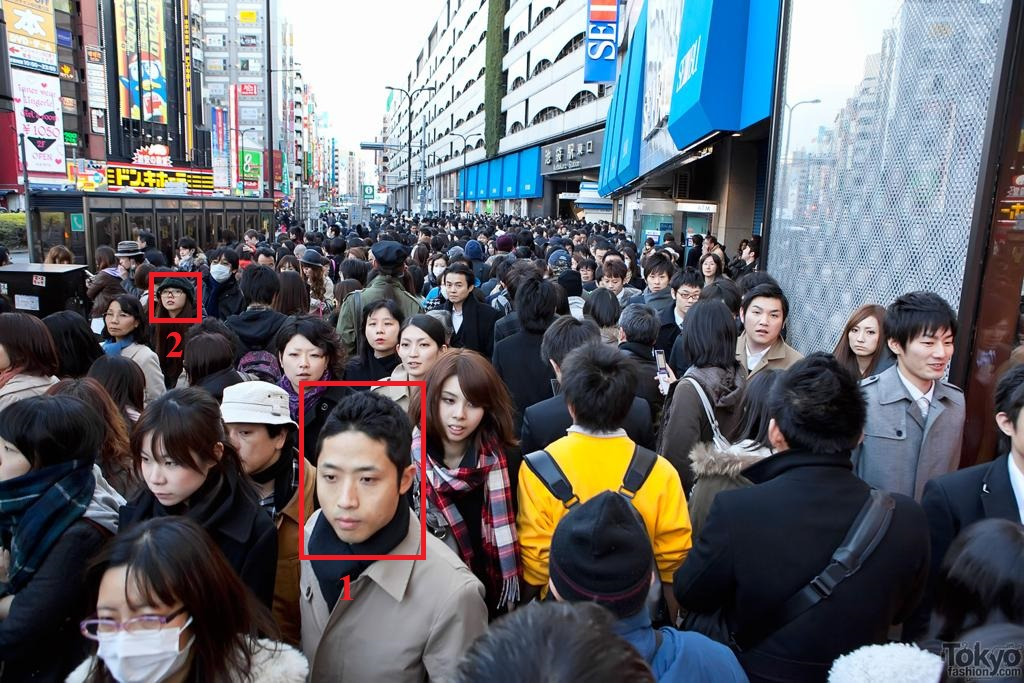
\includegraphics[width=0.4\textwidth]{Picture/problem/part_a_train_IMG_44-annotate-scale.jpg}}
\caption{Scale variation due to perspective distortion. Head in box 1 is bigger than box 2 because people 1 is closer to camera.}
\label{fig:scale}
\end{figure}

Perspective distortion causes people size to variance depending on the camera angle and how far people from the camera is often referred to as a multi-scale problem. The size of people can change between images or vary radically in the same image. The typical CNN model cannot fully adapt to the scale-variance effect. The problem is illustrated in Fig. \ref{fig:scale}. The common solution is a multi-scale feature extraction consists of parallel convolution layers with different receptive field sizes with iconic is multi-column architecture.

Multi-column Convolutional Neural Network (MCNN) \cite{zhang2016single} is among the first model to use multi-columns architecture in crowd counting. MCNN consists of 3 columns, each with different kernel sizes. Feature map output from each column is then concatenated before used to predict the final density map. MCNN was a pioneer to multi-column architecture, in which each column has a different receptive field to copy with a multi-scale problem. Similar works follows \cite{zhang2019crowd, 9053780}. 

However, MCNN fails short when scales vary in the same image. Switch-CNN \cite{sam2017switching} proposed the Switch-classifier, which classifies each image patch to the corresponding CNN column adapts for that specific scale, so does \cite{8965799}. Latter, CAN \cite{liu2019context}, PACNN \cite{shi2019revisiting} merges multi-scale feature with weight-matrix, allowing smoother scale transition across the whole image. 

Another approach is inception-like architecture, inspired from Inception \cite{szegedy2015going}, in which each inception-module, called a multi-scale module, is a mini multi-column convolutional network. The whole network consists of multiple multi-scale modules stack on top of each other, resulting in more scale combinations. SANet \cite{cao2018scale}, MDNet \cite{wang2019multi}, TEDnet \cite{jiang2019crowd}, ADCrowdNet \cite{liu2019adcrowdnet} are notable works. 


Background noise is a challenge in which the background
decreases the performing of count counting algorithm.
Background, which is part of an image scene where there are
no people, impacts the result of the predicted people density
map. Empirical experiments show that density result in the
background zone is not always 0 when it should be. Moreover,
background objects, such as tree leaves, have a pattern similar
to a crowd scene, making it easier to have false positives. Sam et
al. \cite{DBLPconfaaaiSamB18} had clearly documented the effect of background noise in
their work. 

Background noise challenges are tackle, both implicit and explicit approaches. In an explicit approach, authors build a multi-step system, which including a step to remove explicitly remove background from result or input data. Some notable works are: WSRHC \cite{10.1145/3287921.3287980} includes the human-classifier which remove image patches do not contain human; ADCrowdNet \cite{liu2019adcrowdnet} Attention Map Generator segments image into crowd and non-crowd. The implicit approach builds the model so that it is robust to background noise. The common strategies are incorporate contextual information by dilated CNN (CSRNet \cite{li2018csrnet}, CAN \cite{liu2019context}, DMCNN \cite{zhang2019crowd}, \cite{9023874}), combined shallow layers with deep layers (TDF-CNN \cite{DBLPconfaaaiSamB18}, TEDnet \cite{jiang2019crowd}).




% method 
\section{Method} \label{sec:method}


\subsection{Analysis on Compact Convolutional Neural Network}

\begin{figure}[htbp]
\centerline{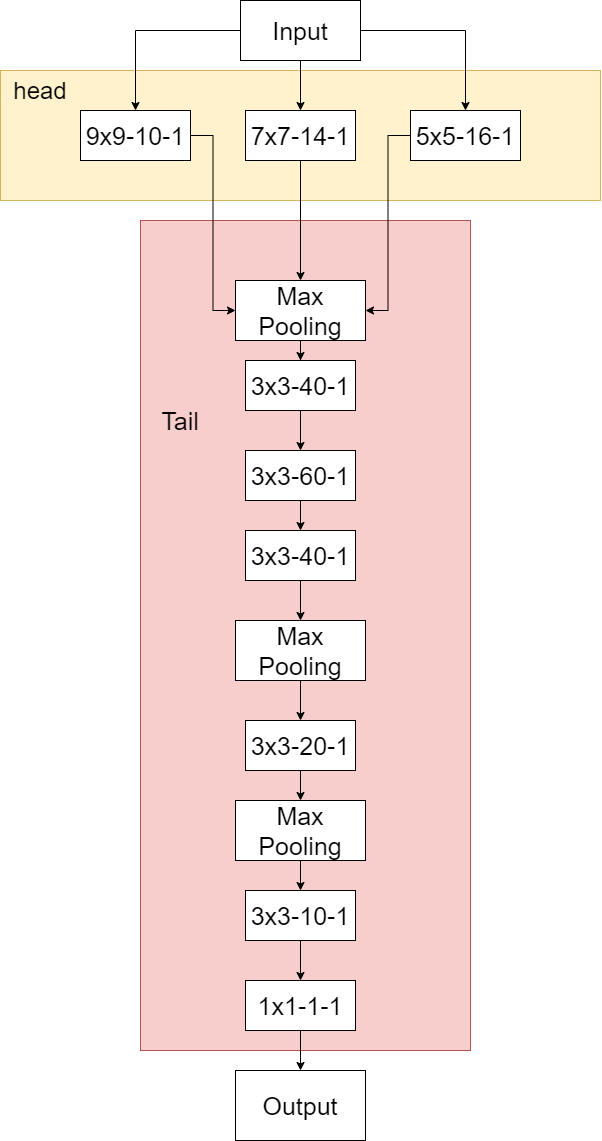
\includegraphics[width=0.4\textwidth]{Picture/proposed/ccnn_original_fix1.png}}
\caption{C-CNN architecture in our re-implementation}
\label{fig:ccnn}
\end{figure}



Despite their performance, state-of-the-art models are complex. C-CNN is a bargain trade performance for efficiency. Fig. \ref{fig:ccnn} is C-CNN from original works \cite{9053780}. We call three branch convolution layer with different kernel size as the "head", and the rest as the tail. CNN module are remark as (kernel size)-(number of filter)-(dilated rate). 

Despite light-weight, C-CNN \cite{9053780} can tackle the problem of scale variation with its "head", consist of 3 parallel CNN with different kernel size. The early feature fusion after first layer not only reduce model complexity but also avoid problem of redundancy in later layer of MCNN \cite{zhang2016single}, which have bean investigate by Li et al. \cite{li2018csrnet}. 
However, there is still room for improvement, as C-CNN \cite{9053780} does not provide any mechanism to alleviate background noise.

% we going Dilated and average pooling
\subsection{Dilated Compact Convolutional Neural Network (DCCNN)} 

\begin{figure}[htbp]
\centerline{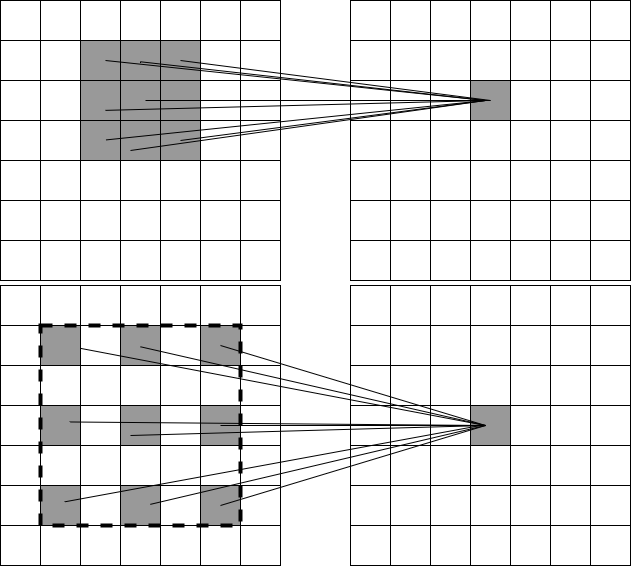
\includegraphics[width=0.4\textwidth]{Picture/example/cnn_vs_dilated_cnn.png}}
\caption{Traditional convolution with dilated rate 1 (top) and dilated convolution with dilated rate 2 (bottom)}
\label{fig:cnn_vs_dilated}
\end{figure}

Dilated convolution with dilated rate n have space n-1 unit between the kernel points. Fig. \ref{fig:cnn_vs_dilated} illustrates dilated convolution with dilated rate 2 (bottom) with traditional convolution (top), whose dilated rate is 1. Dilated convolution can expand the receptive field of without increase kernel size.

Dilated convolution have been proven to conserved spatial context information  and deliver sharper feature map \cite{li2018csrnet}. We hypothesize Dilated convolution can solve the problem of background noise at low cost. Dilated convolution also been widely use in back-end decoder in recent crowd counting model, such as CSRNet \cite{li2018csrnet}, CAN \cite{liu2019context}, DMCNN \cite{zhang2019crowd}, TEDNet \cite{jiang2019crowd}. Inspired by their success, we replace layer all tradition CNN on second layer with Dilated CNN at dilated rate 2. We replace the second and third max-pooling layer into average-pooling to prevent loss of head count in max function \cite{zhang2019crowd}. 

We apply batch normalization \cite{ioffe2015batch} with trainable affine parameters on each CNN layer, including first multi-scale layers. Follow authors work, we add batch normalization before the nonlinearity, in our case, before ReLU activation \cite{agarap2018deep}. 

Fig. \ref{fig:dccnn} is the implementation of our proposed DCCNN.  We hypothesize that DCCNN becomes more robust to background noise, which yields better performance on medium and sparse crowd scenes. 
% Comparing to C-CNN, our proposed model require slightly increase in computation cost and memory due to:

% \begin{itemize}
%     \item 
% \end{itemize}

% \begin{table}[htbp]
% \caption{Experiment result}

\begin{figure}[htbp]
\centerline{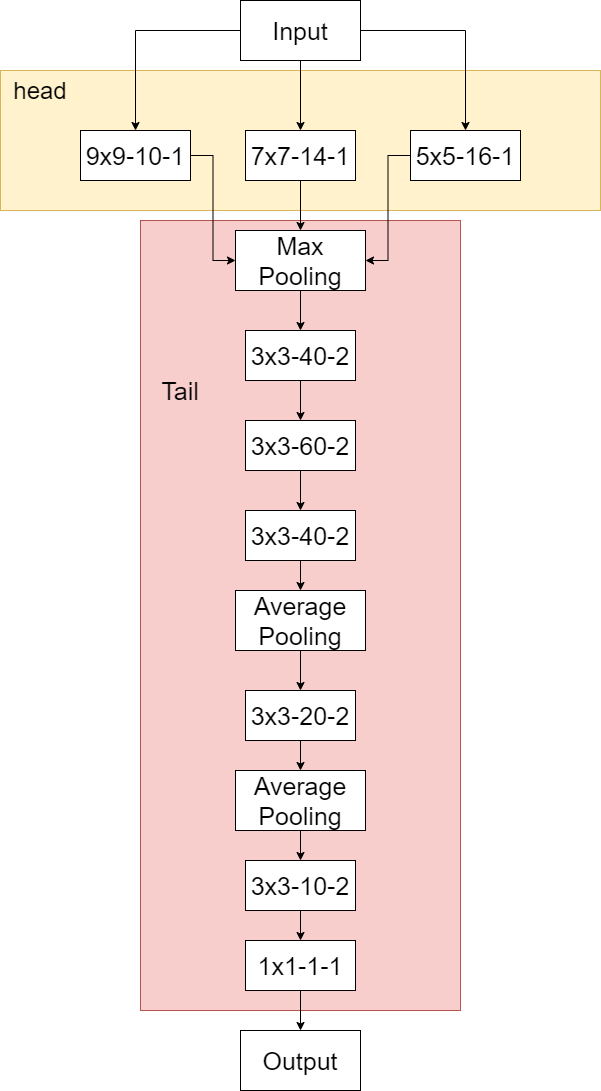
\includegraphics[width=0.4\textwidth]{Picture/proposed/tail13_fix2.png}}
\caption{Our proposed network}
\label{fig:dccnn}
\end{figure}



\subsection{Implementation detail}

\subsubsection{Ground-truth generation} \hfill

For ShanghaiTech Part B dataset \cite{zhang2016single}, we apply Gaussian kernel, original proposed by Lempitsky, \cite{lempitsky2010learning} with $\sigma = 15$ and truncate Gaussian spread at 3 standard deviations. Truncate Gaussian spread help us prevent noise in ground truth density maps, ensure that label at no-human zone is zero. For each image $I_i$, we define ground truth density function as: 

\begin{equation} \label{eq:densit-function}
\forall p \in I_{i}, \quad F_{i}^{0}(p)=\sum_{P \in \mathbf{P}_{i}} \mathcal{N}\left(p ; P, \sigma^{2} \mathbf{1}_{2 \times 2}\right) 
\end{equation}

Where: 
\begin{itemize}
  \item $p$ is pixel
  \item $\mathbf{P}_{i}$ is set of annotated point of image $i$
\end{itemize}

Total people count in image can be acquired by integral \eqref{eq:densit-function}  over whole density map.

% as equation: 

% \begin{equation} \label{eq:count}
% C(I_i) = \sum_{p \in I_{i}} F_{i}(p)
% \end{equation}



\subsubsection{Training detail} \hfill

  To augment ShanghaiTech B dataset, we crop the image into 4 non-overlap patches, each patch we create a copy of its flip over. We limited overlap patches because it might cause overfit \cite{marsden2016fully}. Each full image can generate 8 training patches. 

Inspired by \cite{zhang2019crowd}, we train our model on loss function $L$ composite of Manhattan distance ( $L_1$ loss ) and Euclidean distance ($L_2$ loss): 

\begin{equation}L_2(\Theta)=\frac{1}{N} \sum_{i=1}^{N}\left\|Z\left(X_{i} ; \Theta\right)-Z_{i}^{G T}\right\|^{2}\end{equation}

\begin{equation}L_1(\Theta)=\frac{1}{N} \sum_{i=1}^{N}\left\|Z\left(X_{i} ; \Theta\right)-Z_{i}^{G T}\right\|\end{equation}

\begin{equation}
    L(\Theta) = \frac{1}{2}L_1(\Theta) + \frac{1}{2}L_2(\Theta)
\end{equation}

\begin{itemize}
  \item $\Theta$ is set of model parameters
  \item $Z\left(X_{i} ; \Theta\right)$ is predicted density map from image $I_i$
  \item $Z_{i}^{G T}$ is ground truth density map generated from annotated head of image $I_i$
\end{itemize}

 
 We train the model end-to-end with batch size of 40 patches and AdamW optimizer \cite{loshchilov2017decoupled} with learning rate of 0.001 and weight-decay 0.1. The following source code \footnote{https://github.com/ttpro1995/crowd\_counting\_framework} and setting \footnote{train\_script/learnstuff/l1/adamw1\_bigtail13i\_t1\_shb.sh} can reproduce result in approximately 8 hours of training.



%% TODO







% exp
\section{Experiment}

\subsection{Evaluation metric}

% While we training and compute loss function for backpropagation on generated ground-truth density map,

From the predicted density map, we acquired predicted count by integral the density map over the whole image (i.e., sum the predicted density map matrix). Then from the predicted count and annotated count, compute Mean Absolutately Error (MAE), Mean Square Error (MSE) 

\begin{equation}M A E=\frac{1}{N} \sum_{i=1}^{N}\left|C_{i}^{e t}-C_{i}^{g t}\right|\end{equation}

\begin{equation}M S E=\sqrt{\frac{1}{N} \sum_{i=1}^{N}\left(C_{i}^{e t}-C_{i}^{g t}\right)^{2}}\end{equation}

\subsection{ShanghaiTech B}

Table \ref{tab:experiment-result} show experiment result and trainable parameter of our proposed method comparing to C-CNN. The increase in parameter size due to learnable affine parameters in batch normalization.  

\begin{table}[htbp]
\caption{\label{tab:experiment-result}  Experiment result}
\begin{center}
\begin{tabular}{|c|c|c|}
\hline
\textbf{}&\multicolumn{2}{|c|}{\textbf{ShanghaiTech B}}\\
\hline
\textbf{Model} & \textbf{\textit{MAE}}& \textbf{\textit{MSE}} \\
\hline
C-CNN & 14.9 & 22.1   \\
\hline
Ours & 12.2 & 21.9  \\
\hline

\end{tabular}

\end{center}
\end{table}


% % benchmark FPS
% \begin{table}[htbp]
% \caption{\label{tab:benchmark}  Benchmark}
% \begin{center}
% \begin{tabular}{|c|c|c|}
% \hline
% \textbf{}&\multicolumn{2}{|c|}{\textbf{ShanghaiTech B}} \\
% \hline
% \textbf{Model} & \textbf{\textit{Average time (seconds)}}& \textbf{\textit{FPS}} \\
% \hline
% C-CNN (authors) &   & 104.16    \\
% \hline
% C-CNN (our implementation) & 7.15 &  44.5    \\
% \hline
% Ours & 6.95 & 45.7 \\
% \hline
% % \multicolumn{3}{l}{$^{\mathrm{a}}$ Parameter size in our implementation.}
% \end{tabular}

% \end{center}
% \end{table}

\subsection{Benchmark}

% TODO average time, parameter size 
% we talk about resource consumption here

We run benchmark our re-implementation C-CNN \cite{9053780} and our proposed DCCNN on predefined ShanghaiTech B test set, total 318 test images, on the same hardware. Models are run on inference mode on a batch size of 1. We count the number of trainable parameters and measure total running time in second. Benchmark results are summarized in Table \ref{tab:benchmark-result}. Running times are averaged from multiple runs of same setting. Unfortunately, we cannot reproduce C-CNN benchmark of original authors \cite{9053780} (104.16 FPS) due to hardware limitations. 

\begin{table}[htbp]
\caption{\label{tab:benchmark-result}  Benchmark}
\begin{center}
\begin{tabular}{|c|c|c|c|}
\hline
\textbf{}&\multicolumn{2}{|c|}{\textbf{ShanghaiTech B}}&\textbf{Parameter} \\
\cline{1-3}
\textbf{Model} & \textbf{\textit{ Time (seconds) }}& \textbf{\textit{FPS}}&\textbf{Size} \\
\hline
C-CNN (authors) &  &  104.16 & 0.07M \\
\hline
C-CNN$^{\mathrm{a}}$  & 6.95482 & 45.72 & 72509   \\
\hline
Ours &  7.15093 & 44.47 & 73009 \\
\hline
\multicolumn{4}{l}{$^{\mathrm{a}}$ Our re-implementation of C-CNN}
\end{tabular}

\end{center}
\end{table}

Comparing to C-CNN \cite{9053780}, our DCCNN require more computing resource, however due to: 
\begin{itemize}
    \item Batch normalization: 500 trainable affine parameters, more computation
    \item 2 layer of average pooling instead of max pooling: more computation 
\end{itemize}

\section{Conclusion} \label{sec:conclusion}

In this paper, we proposed DCCNN, a lightweight model with mechanisms to tackle both perspective distortion and background noise challenges. By replacing the tail part of the model with dilated convolution and two max pooling with average pooling, DCCNN can better incorporate spatial information. As a result, DCCNN delivered sharper density maps with less noise. We demonstrated our model in medium and spared dataset ShanghaiTech part B \cite{zhang2016single} with C-CNN \cite{9053780} to compare their performance and efficiency.

% In this work, we proposed utilized dilated convolution to upgrade C-CNN \cite{9053780} into DCCNN. DCCNN is as light-weight as C-CNN. However, the performance boost on medium and spares crowd scene is significant. 



% \begin{table}[htbp]
% \caption{Table Type Styles}
% \begin{center}
% \begin{tabular}{|c|c|c|c|}
% \hline
% \textbf{Table}&\multicolumn{3}{|c|}{\textbf{Table Column Head}} \\
% \cline{2-4} 
% \textbf{Head} & \textbf{\textit{Table column subhead}}& \textbf{\textit{Subhead}}& \textbf{\textit{Subhead}} \\
% \hline
% copy& More table copy$^{\mathrm{a}}$& &  \\
% \hline
% \multicolumn{4}{l}{$^{\mathrm{a}}$Sample of a Table footnote.}
% \end{tabular}
% \label{tab1}
% \end{center}
% \end{table}

% \section{}

\section*{Acknowledgment}

This research is funded by Vietnam National University Ho Chi Minh City (VNUHCM) under grant no. B2018-18-01.

\bibliographystyle{IEEEtran}
\bibliography{IEEEabrv,IEEEfull.bib}



\end{document}
